\section{Pattern Optimization}
\begin{frame}{Goal}
    \begin{itemize}
        \item For each grid cell, find a pattern with $Y, \nu \approx Y^*, \nu^*$ from
   material optimization.
 \item I.e. "invert" the homogenization procedure
 \item Could sample the 9+ dimensional pattern parameter space and find closest
   tensor...
 \item .. but space is huge, $N^P$ sample points ($N$ samples per param, $P$ params)
\end{itemize}
\end{frame}

\begin{frame}{Shape Optimization}
    \begin{itemize}
\item Ideally we can tune the elasticity tensor with an optimization:
    $$ \min_p \norm{C - C^*}^2 $$
\item $p$ controls {\bf shape} of microstructure! How can we optimize it?
\item Use the ``shape derivative''
    \begin{figure}
        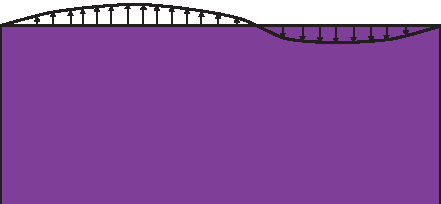
\includegraphics[width=.35\textwidth]{Images/vn.pdf}
        $v_n$
    \end{figure}
        $$ J(\omega) = \norm{C(\omega) - C^*}^2 $$
        $$
        \delta J[v_n](\omega) = \lim_{\epsilon \to 0} \frac{J(\omega) - J(\omega_{\text{perturbed by $\epsilon v_n$}})}{\epsilon}
        $$
    \end{itemize}
\end{frame}

\begin{frame}{Shape Optimization}
    \begin{itemize}
        \item Amazingly, the closed form of each entry of the homogenized elasticity tensor can be
              shape differentiated
                $$
                \delta C^H_{ijkl}[v_n] = \frac{1}{|Y|} \int_{\partial \omega} \left[(e^{ij} + e({\bf w}^{ij})) : C : (e^{kl} + e({\bf w}^{kl}))\right] v_n \dA({\bf y})
                $$
            \item If we know the normal velocity caused by each pattern parameter, $p_a$, plug it in (chain rule):
              $$
              \pder{C^H_{ijkl}}{p_a} =
              \frac{1}{|Y|} \int_{\partial \omega} \left[(e^{ij} + e({\bf w}^{ij})) : C : (e^{kl} + e({\bf w}^{kl}))\right] {\bf v}_{p_a} \cdot {\bf \hat{n}} \dA({\bf y})
              $$
    \end{itemize}
\end{frame}

\begin{frame}{Other Objectives}
    \begin{itemize}
        \item It might be better to optimize a different objective than fitting the elasticity tensor.
        \begin{itemize}
            \item Fit compliance tensor
                $$ min_p \norm{C^{-1} - {C^*}^{-1}}^2 $$
            \item Fit Poisson ratio
                $$ min_p \norm{\nu - \nu^*}^2 $$
        \end{itemize}
        \item Gradients of these can be computed using chain rule.
    \end{itemize}
\end{frame}

\begin{frame}{Example}
\end{frame}
